\begin{usecase}{Extract Events from WhatsApp}
  \ucbasicinfo{High}{Regular}
  \ucshortdescription{System monitors WhatsApp messages through whatsapp-web.js, analyzes conversations using OpenAI API compatible LLMs to detect events, and adds confirmed events to a dedicated WhatsApp calendar via CalDAV.}
  \uctrigger{A non-group message is sent to or from the connected WhatsApp account.}
  \ucactors{WhatsApp, LLM Service, CalDAV Server}{}
  \ucpreconditions{
    \begin{itemize}
      \item WhatsApp account must be connected via whatsapp-web.js
      \item RabbitMQ message queues must be operational
      \item OpenAI API compatible LLM must be configured
      \item CalDAV server must be accessible
    \end{itemize}
  }
  \ucrelationships{N/A}{N/A}{N/A}
  \ucinputsoutputs{
    \begin{itemize}
      \item \textbf{WhatsApp message details} (Source: whatsapp-web.js)
      \item \textbf{Message history from database} (Source: System Database)
    \end{itemize}
  }{
    \begin{itemize}
      \item \textbf{Event analysis result} (JSON with status and details)
      \item \textbf{Calendar event} (Added to CalDAV server)
      \item \textbf{Push notification} (To user's devices)
    \end{itemize}
  }
  \ucmainflow{
    \begin{enumerate}
      \item System receives a non-group message via whatsapp-web.js client
            \ucinfo{Message details including sender, body, timestamp are captured}
      \item Message is published to RabbitMQ queue for processing
            \ucinfo{Message consumer retrieves message context from database}
      \item LLM analyzes message context with specialized prompt
            \ucinfo{Analysis determines if message contains event and its status (\textit{NO\_EVENT}, \textit{HAS\_EVENT\_BUT\_NOT\_CONFIRMED}, \textit{HAS\_EVENT\_AGREED}, \textit{HAS\_EVENT\_DENIED})}
      \item If event is detected and agreed upon:
            \begin{itemize}
              \item Event is published to calendar queue
              \item CalDAV credentials are retrieved
              \item Event is added to WhatsApp Events calendar on CalDAV server
              \item Push notification is sent to user's devices
            \end{itemize}
    \end{enumerate}
  }
  \ucalternateflows{
    \begin{itemize}
      \item If event is detected but not confirmed, system continues monitoring chat
      \item If event is denied, chat history is cleared
    \end{itemize}
  }
  \ucexceptions{
    \begin{itemize}
      \item LLM analysis errors are logged for debugging
      \item Message processing failures trigger message requeuing
      \item WhatsApp client disconnections trigger automatic cleanup
      \item CalDAV server connection failures are handled gracefully
    \end{itemize}
  }
  \ucconclusion{Event is successfully extracted, added to CalDAV calendar, and user is notified}
  \ucpostconditions{
    \begin{itemize}
      \item Event is added to WhatsApp Events calendar on CalDAV server
      \item User receives push notification
      \item Chat history is cleared after successful processing
    \end{itemize}
  }
  \ucbusinessrules{
    \begin{itemize}
      \item Group messages are ignored
      \item Events require explicit agreement to be added
      \item WhatsApp Events calendar has a dedicated format
      \item Push notifications include event details for user verification
    \end{itemize}
  }
  \ucspecialrequirements{
    \begin{itemize}
      \item whatsapp-web.js client for WhatsApp integration
      \item RabbitMQ for message queuing
      \item OpenAI API compatible LLM service
      \item CalDAV server (Baikal) for calendar storage
      \item Push notification service configuration
      \item Encryption keys for securing sensitive data at rest:
            \begin{itemize}
              \item WhatsApp messages encryption key
              \item CalDAV credentials encryption key
            \end{itemize}
    \end{itemize}
  }
\end{usecase}

The ``Extract Events from WhatsApp Sequence Diagram'', shown in \textbf{Figure~\ref{fig:seq/extract-events-whatsapp}}, illustrates the event extraction workflow through a message queue architecture. The system consists of several components working together, with a focus on security through encryption at rest:

\begin{itemize}
  \item The WhatsApp Service (using whatsapp-web.js) monitors non-group messages
  \item RabbitMQ message queues handle asynchronous processing:
        \begin{itemize}
          \item Message Queue for WhatsApp messages
          \item Calendar Queue for confirmed events
        \end{itemize}
  \item Message Consumer processes messages and coordinates with the LLM
  \item Calendar Consumer handles CalDAV integration
  \item Push notification service for user updates
  \item Database stores sensitive data encrypted at rest:
        \begin{itemize}
          \item WhatsApp messages are encrypted with a dedicated key
          \item CalDAV credentials are encrypted with a separate key
        \end{itemize}
\end{itemize}

The workflow operates as follows:
\begin{enumerate}
  \item The WhatsApp Service filters out group messages and publishes individual messages to a RabbitMQ queue
  \item The Message Consumer:
        \begin{itemize}
          \item Retrieves the message context from the database
          \item Sends the context to the LLM Service for analysis
          \item Handles different event statuses returned by the LLM:
                \begin{itemize}
                  \item \textit{NO\_EVENT}: No action needed
                  \item \textit{HAS\_EVENT\_BUT\_NOT\_CONFIRMED}: Continues monitoring
                  \item \textit{HAS\_EVENT\_DENIED}: Clears chat history
                  \item \textit{HAS\_EVENT\_AGREED}: Publishes to calendar queue
                \end{itemize}
        \end{itemize}
  \item When an event is agreed upon, the Calendar Consumer:
        \begin{itemize}
          \item Retrieves encrypted CalDAV credentials from database
          \item Initializes the WhatsApp Events calendar on CalDAV server if needed
          \item Adds the event directly to the calendar via CalDAV
          \item Sends a push notification to user's devices
          \item Clears the chat history from database
        \end{itemize}
\end{enumerate}

This queue-based architecture ensures reliable message processing and proper separation of concerns between message analysis and calendar integration. The system's ability to handle different event statuses allows for natural conversation flow while maintaining accurate event tracking. All sensitive data, including WhatsApp messages and CalDAV credentials, are encrypted at rest in the database, while the actual calendar events are stored securely on the CalDAV server.

\begin{figure}[!h]
  \centering
  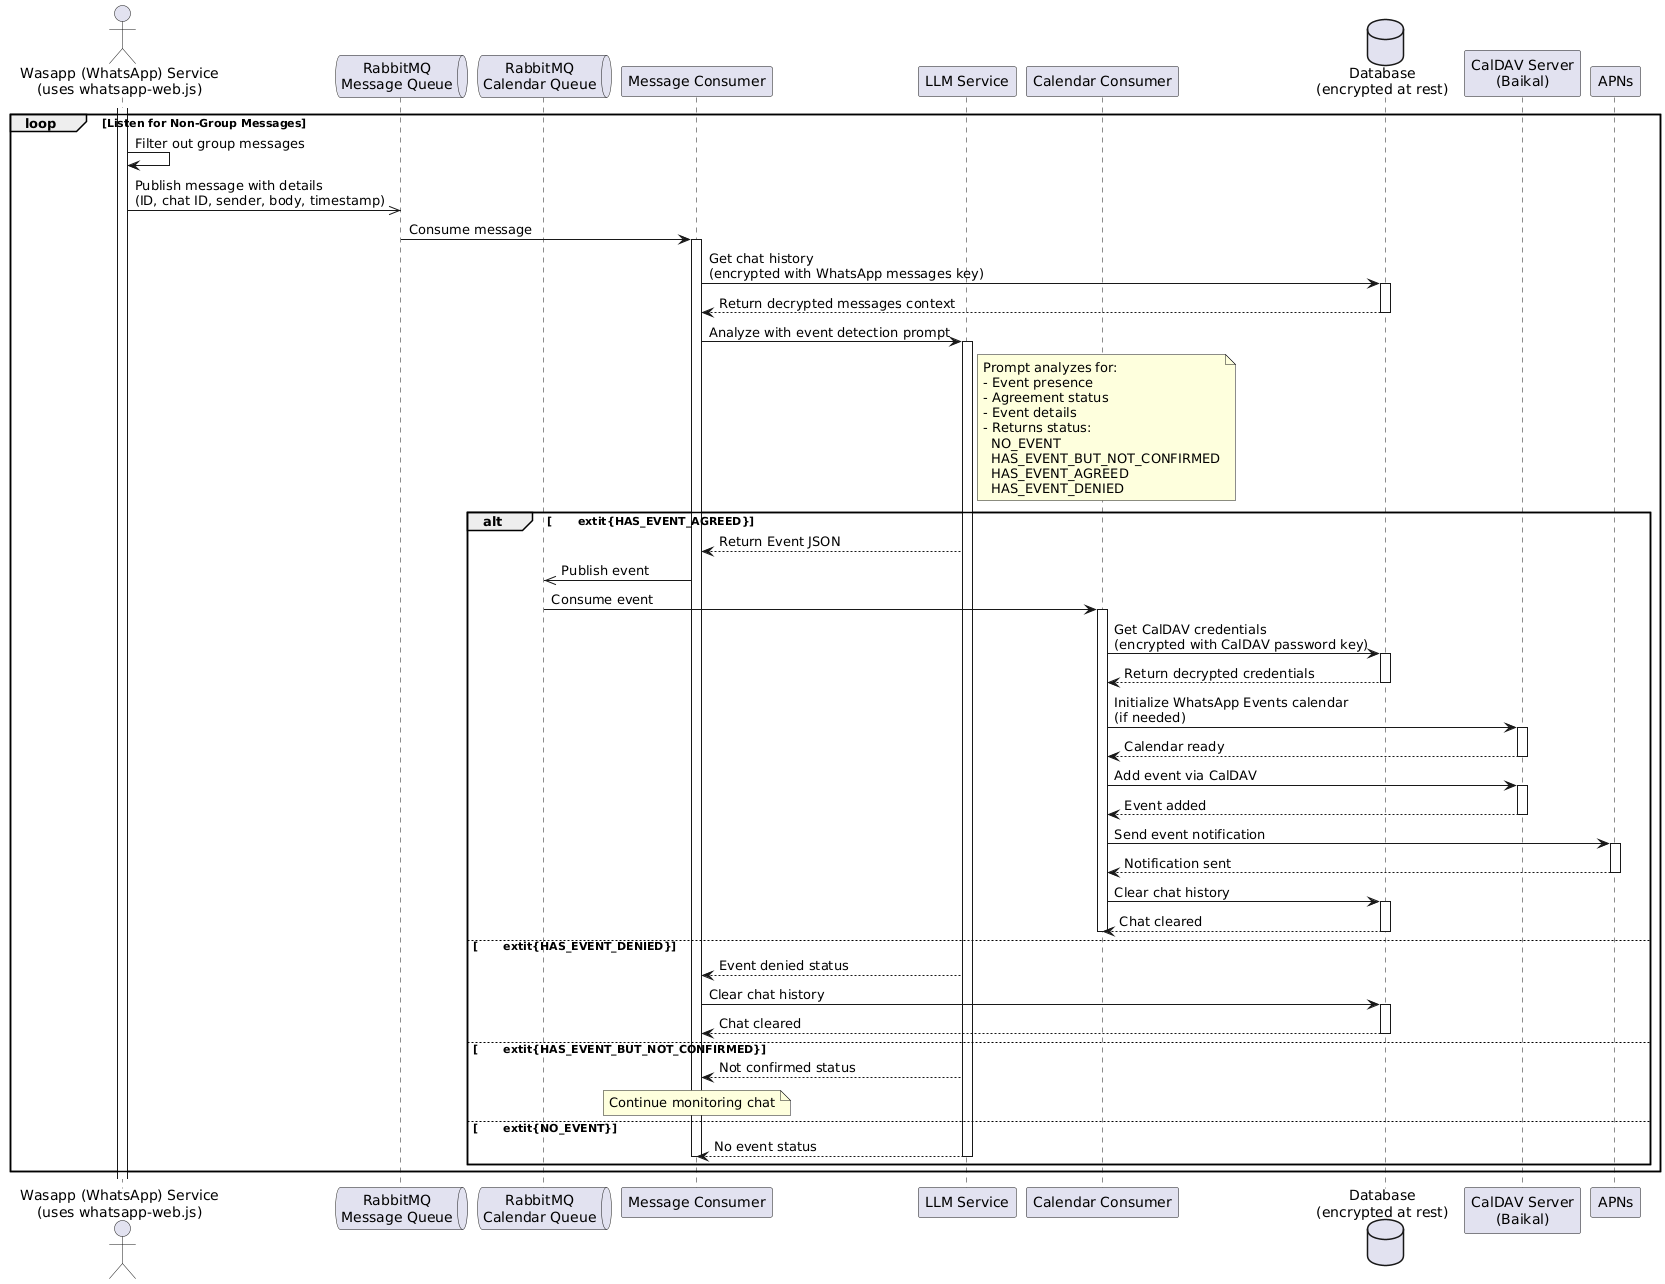
\includegraphics[width=\textwidth]{images/docs/diagrams/sequence-diagrams/all-sequence-diagrams/Extract Events from WhatsApp.png}
  \caption{Extract Events from WhatsApp Sequence Diagram}
  \label{fig:seq/extract-events-whatsapp}
\end{figure}
